\chapter{Core concepts}

After analyzing several ORMs, we discovered significant differences among them, yet their core purpose remains identical. The primary objective is consistently retrieving data through queries and transforming database records into application objects based on a defined set of mapping rules.

\begin{figure}[H]
  \centering
  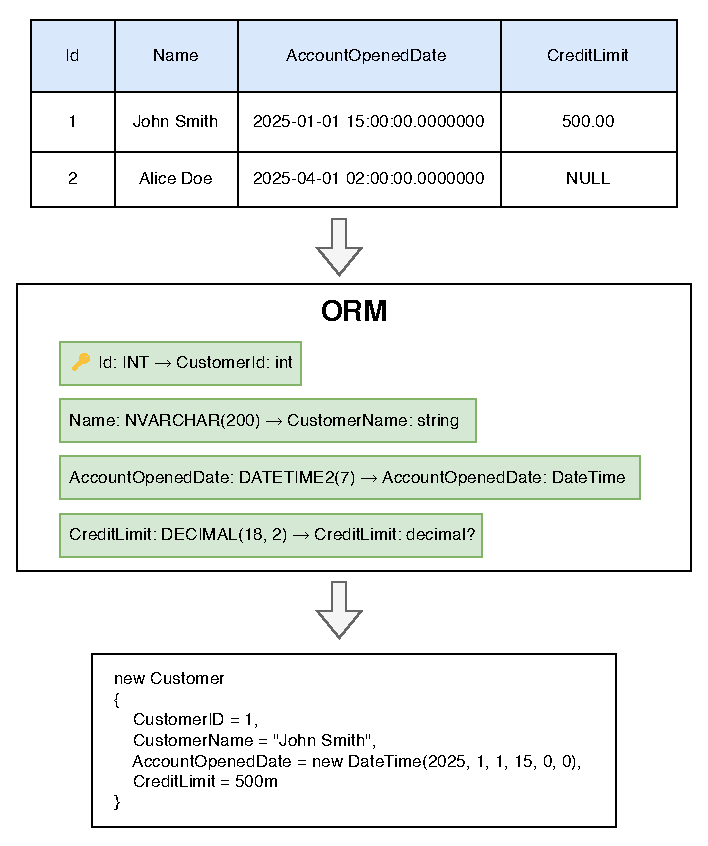
\includegraphics[height=1\textwidth]{thesis/img/thesis/03_orm_transformation.drawio.pdf}
  \caption{The process of converting database records to application objects using ORM with defined rules.}
  \label{fig:db_to_orm}
\end{figure}

The transformation is illustrated in \autoref{fig:db_to_orm}. The database record is processed through an ORM, represented here as a black box containing predefined mapping rules, ultimately converting the data into a strongly typed C\# object.

Despite their common goals, we observed significant performance differences during the evaluation in \autoref{sec:perf_eval}. For instance, query \hyperref[query:d3]{D3}, testing retrieval of one-to-many optional relationships, took over 2.5 seconds in EF Core. In contrast, the same query executed with linq2db completed in just 91 milliseconds--a performance improvement of more than twenty times. Clearly, performance differences among ORMs can be substantial.

Typically, developers stick to using a single ORM per application, mainly to avoid complexity. However, combining multiple ORMs can be beneficial, particularly in performance-critical areas. For example, as we noted in \autoref{sec:feat_dapper}, Dapper's creators explicitly suggest using it alongside another macro ORM to boost read performance where necessary. Nonetheless, employing multiple ORMs on the same database tables may introduce issues like data inconsistencies, particularly during write operations. Read operations do not modify the state of the database, and we will only work with read operations in this work. Ensuring consistency remains a developer's responsibility when mixing ORMs.

Currently, converting queries from one ORM to another is challenging and typically requires manual intervention. Our approach will focus on automating this conversion process. We propose creating an abstraction that unifies entities, mappings, and queries into an intermediate representation, enabling efficient conversion between different ORM frameworks.

\section{Translation}

In a .NET application, queries depend not only on the query statements themselves but also on entities and their respective mappings. While entities are always represented as C\# classes, mappings vary significantly. We have encountered mapping defined via attributes, fluent code syntax, and even XML files. Despite these syntactical differences, the conceptual goal remains the same. We have to explicitly instruct the ORM how entities map to database tables, including data types, constraints, and relationships. To effectively automate query translation, we must begin with identifying common patterns across these diverse mapping strategies.

Querying approaches differ similarly, primarily between raw SQL and strongly-typed LINQ queries. RepoDB introduces a third variant---lambda functions---but these functions can be viewed as a very limited subset of LINQ and therefore we will not consider them separately. Regardless of initial query method, all queries eventually get translated into SQL statements executed by the database. This observation makes SQL a logical basis for a unified abstraction layer.

By creating a common abstraction over entities, mappings, and queries, we achieve a unified intermediate representation suitable for translation between different ORMs. Implementing this intermediate representation significantly simplifies the translation task. Instead of requiring $N^2 - N$ direct conversions (each ORM to every other ORM, excluding self-conversions), we reduce the effort to just $2N$ conversions---one into the intermediate representation and one out for each ORM. Additionally, not every conversion direction needs full support. For instance, translating from a deprecated ORM might be useful for migrations, but translating into it may be unnecessary.

Leveraging this approach, we will design and implement a tool that automates query conversion and facilitates easy performance comparisons across different ORM frameworks.

\section{User interaction}
Input into the conversion tool will be \textbf{entity}, \textbf{mapping} and a \textbf{query}. Not all ORMs require or even support mapping, and there are different formats. So each ORM will have defined which parts it accepts. Input framework can be either auto-detected or manually selected by the user. Upon selection, multiple inputs with a description will appear.

As an example in \autoref{fig:orm_to_abstract}, the user selects Entity Framework Core as the source ORM. Given we support only attribute mapping, two inputs will be shown. One for an attributed entity and a second for a LINQ query. After user confirms 

\begin{figure}[H]
  \centering
  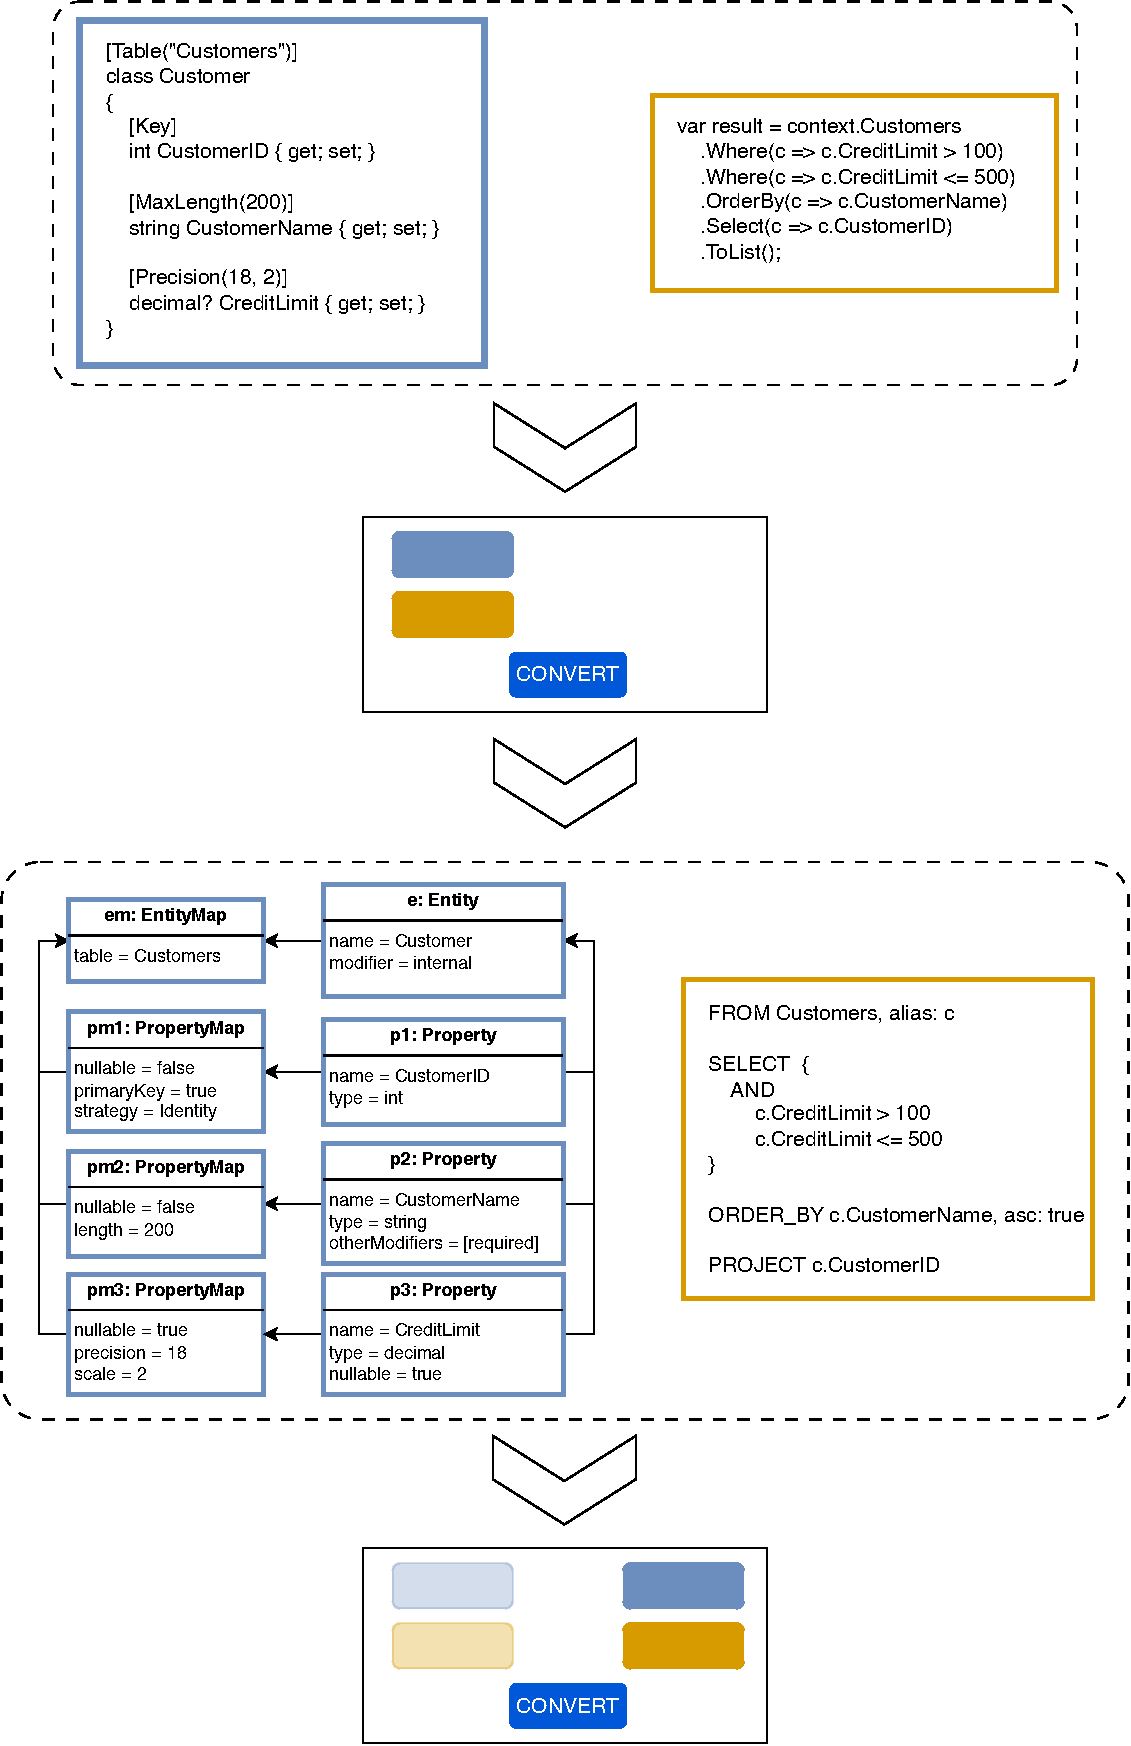
\includegraphics[width=\textwidth]{thesis/img/thesis/03_user_interaction.drawio.pdf}
  \caption{An example of entity and query being converted into abstract representation. User inputs EF Core entity and LINQ query. Our tool converts it to abstract representation, which in turn can be translated into any user selected ORM.}
  \label{fig:orm_to_abstract}
\end{figure}

\section{Advisor}
TODO advisor